\documentclass{beamer}
%
% Choose how your presentation looks.
%
% For more themes, color themes and font themes, see:
% http://deic.uab.es/~iblanes/beamer_gallery/index_by_theme.html
%
\mode<presentation>
{
  \usetheme{default}      % or try Darmstadt, Madrid, Warsaw, ...
  \usecolortheme{default} % or try albatross, beaver, crane, ...
  \usefonttheme{default}  % or try serif, structurebold, ...
  \setbeamertemplate{navigation symbols}{}
  \setbeamertemplate{caption}[numbered]
  \setbeamertemplate{footline}[frame number]
} 

\usepackage[english]{babel}
\usepackage[utf8x]{inputenc}
\usepackage{dirtree}
\usepackage{listings}
\usepackage{courier}

\title[2016-04-04-offline-pr-overview]{Big Data techniques and \\ applying them to high energy physics}
\author{Jim Pivarski}
\institute{Princeton University -- DIANA}
\date{April 4, 2016}

\xdefinecolor{darkblue}{rgb}{0.1,0.1,0.7}
\definecolor{mygreen}{rgb}{0,0.6,0}
\definecolor{mygray}{rgb}{0.5,0.5,0.5}
\definecolor{mymauve}{rgb}{0.58,0,0.82}

\lstset{ %
  backgroundcolor=\color{white},   % choose the background color
  basicstyle=\ttfamily\scriptsize,        % size of fonts used for the code
  breaklines=true,                 % automatic line breaking only at whitespace
  captionpos=b,                    % sets the caption-position to bottom
  commentstyle=\color{mygreen},    % comment style
  escapeinside={\%*}{*)},          % if you want to add LaTeX within your code
  keywordstyle=\color{blue},       % keyword style
  stringstyle=\color{mymauve},     % string literal style
}

\begin{document}

\begin{frame}
  \titlepage
\end{frame}

% Uncomment these lines for an automatically generated outline.
%\begin{frame}{Outline}
%  \tableofcontents
%\end{frame}

\begin{frame}{How did I end up giving this talk?}
\begin{itemize}
\item I'm a CMS physicist, contributed to muon alignment in Run-1 commissioning and early exotica searches.
\item Spent the next five years as a data science consultant:
\begin{itemize}
\item Helped commercial clients analyze data with Big Data technologies: Hadoop, Spark, NoSQL, etc.
\item Some statistics, but more software and data pipelines.
\end{itemize}
\end{itemize}

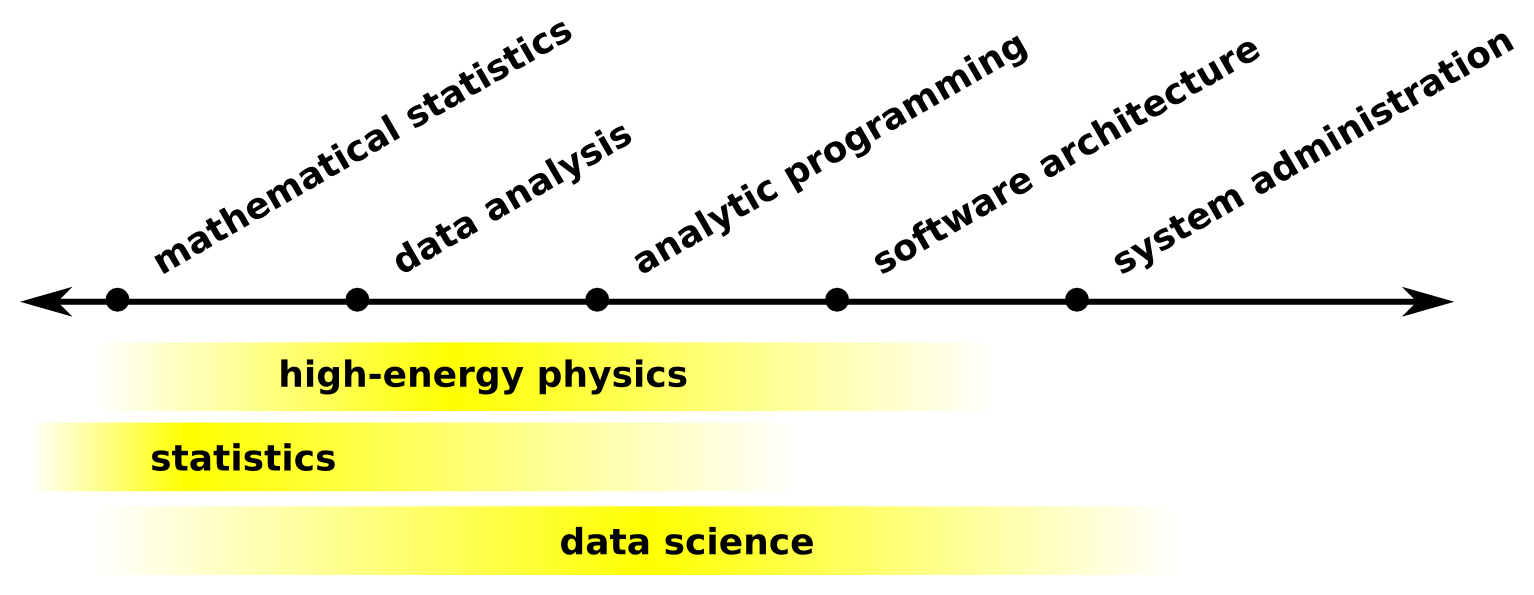
\includegraphics[width=\linewidth]{spectrum_of_data_science.png}

\begin{itemize}
\item I'm part of a project to introduce Big Data tools to HEP: Project DIANA.
\end{itemize}
\end{frame}

\begin{frame}{Differences between HEP and the Big Data world}
\begin{columns}
\column{0.5\linewidth}
One integrated toolkit: ROOT. Compared to a ``city'' in the User's Guide.

\column{0.5\linewidth}
Many competing frameworks and data formats that interoperate: ``city-states?''
\end{columns}

\vfill
\uncover<2->{\hrulefill}

\vfill
\begin{columns}<2->
\column{0.5\linewidth}
C++ for data plumbing and (increasingly) Python for end-user analysis.

\column{0.5\linewidth}
Java for data plumbing and (mostly) R, Python, and SQL for analysis.
\end{columns}

\vfill
\uncover<3->{\hrulefill}

\vfill
\begin{columns}<3->
\column{0.5\linewidth}
Extensive distributed filtering \\ and data transformations \\ (``map'' from map-reduce).

\column{0.5\linewidth}
Extensive distributed map {\it and} reduce: regrouping data from one attribute to another.
\end{columns}

\vfill
\uncover<4->{\hrulefill}

\vfill
\begin{columns}<4->
\column{0.5\linewidth}
Data analysis mostly written imperatively: for loops, break/continue statements.

\column{0.5\linewidth}
Increasing use of functional primitives: map, filter, flatMap, reduce, aggregate.
\end{columns}
\end{frame}

\vfill
\begin{frame}{}


\end{frame}





%% \begin{frame}[fragile]
%% \frametitle{Map-reduce}

%% Hadoop executes two sets of independent, identical processors:
%% \begin{itemize}
%% \item Mappers, which transform each input to a $\langle$key, value$\rangle$ pair.
%% \item Reducers, each operates on all values that have a given key.
%% \end{itemize}

%% \vspace{-0.1 cm}
%% \begin{columns}
%% \column{0.5\linewidth}
%% \begin{lstlisting}[frame=single]
%% def mapper($webpage$):
%%   for $word$ in $webpage$.split():
%%     yield ($word$, $webpage$)
%% $$
%% \end{lstlisting}
%% \column{0.58\linewidth}
%% \begin{lstlisting}[frame=single]
%% def reducer($word$, $webpages$):
%%   searchIndex[$word$] = {}
%%   for $webpage$ in $webpages$:
%%     searchIndex[$word$].add($webpage$)
%% \end{lstlisting}
%% \end{columns}

%% The system groups data by key in an optimized way (independent partial sorts followed by merge, minimizing network bandwidth).

%% \vspace{0.2 cm}
%% \mbox{ } \hfill 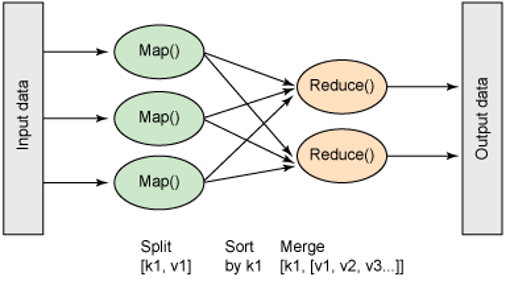
\includegraphics[width=0.6\linewidth]{mapreduce-diagram-by-ibm.png} \hfill \mbox{ }
%% \end{frame}

%% \begin{frame}[fragile]
%% \frametitle{Potential application in physics}

%% Most physics analyses apply the same function to all \mbox{events independently.\hspace{-1 cm}}

%% However, alignment and calibration are more tightly coupled:
%% \begin{itemize}
%% \item Alignment residuals must be re-indexed from tracks to subdetectors.
%% \item Calibration responses must be re-indexed from $\pi^0$s to subdetectors.
%% \end{itemize}

%% \begin{lstlisting}[frame=single]
%% def mapper($event$):
%%     for $track$ in $event$:
%%         for $hit$ in $track$:
%%             key = $hit$.subdetector()
%%             residual = $track$.projection($hit$) - $hit$.pos()
%%             yield (key, residual)
%% \end{lstlisting}

%% \begin{lstlisting}[frame=single]
%% def reducer($subdetector$, $residuals$):
%%     numer = 0
%%     denom = 0
%%     for $residual$ in $residuals$:
%%         numer = numer + $residual$
%%         denom = denom + 1
%%     >move>($subdetector$, numer/denom)  # shift by residual mean
%% \end{lstlisting}

%% Map-reduce can be applied to {\it one iteration} of alignment or calibration.
%% \end{frame}

%% \begin{frame}[fragile]
%% \frametitle{Alignment example in Spark}

%% \begin{lstlisting}
%% @case class Ratio(numer, denom):
%%     def add(self, other):
%%         return >Ratio>(self.numer + other.numer,
%%                      self.denom + other.denom)
%%     def value(self):
%%         return self.numer / self.denom

%% def makePair($track$, $hit$):
%%     key = $hit$.subdetector()
%%     residual = $track$.projection($hit$) - $hit$.pos()
%%     return (key, >Ratio>(residual, 1))
%% \end{lstlisting}

%% \begin{lstlisting}[frame=single]
%% $tracks$.cache()   # tells Spark to keep tracks in memory

%% for $iteration$ in range(100):
%%     keyValuePairs =
%%         $tracks$.flatMap(lambda $track$: $track$.hits.map(
%%                          lambda $hit$: >makePair>($track$, $hit$)))

%%     corrections =
%%         keyValuePairs.reduceByKey(lambda r1, r2: r1.>add>(r2))
%%                      .mapValues(lambda r: r.>value>())

%%     corrections.foreach(>move>)
%% \end{lstlisting}
%% \end{frame}

%% \begin{frame}
%% \frametitle{Language choice}

%% Everything mentioned so far was written in Java (or Scala or Clojure) with hooks for Python and R. Little support for C/C++. Why is that?

%% \vfill
%% \uncover<2->{\renewcommand{\arraystretch}{1.0} \begin{tabular}{>{\raggedright}p{0.3\linewidth} >{\raggedright}p{0.3\linewidth} >{\raggedright\arraybackslash}p{0.3\linewidth}}
%% \textcolor{darkblue}{C/C++} & \textcolor{darkblue}{JVM (Java et al)} & \textcolor{darkblue}{Python and R} \\
%% \vspace{-0.2 cm} Hardest to debug. Mixes analysis with low-level concerns. & \vspace{-0.2 cm} Human-readable internals, stack traces, runtime types. & \vspace{-0.2 cm} Interactive prompt! Everything can be inspected at runtime. \\
%% \uncover<3->{Fastest, raw machine access, \mbox{static bytecode,\hspace{-1 cm}} manual memory management.} & \uncover<3->{Medium speed, dynamic optimizer.} \only<3-4>{Garbage collector is fast but pauses.} \only<5>{\fbox{\begin{minipage}{\linewidth} \raggedright Garbage collector is fast but pauses. \end{minipage}}} & \uncover<3->{Slowest, though performance-critical code is external.} \\
%% \uncover<4->{Used by physicists (and cybersecurity).} & \uncover<4->{Used for large-scale business analytics; suited to networking.} & \uncover<4->{Used by statisticians and data scientists for laptop-analyses.}
%% \end{tabular}}
%% \end{frame}

%% \begin{frame}[fragile]
%% \frametitle{Immutable data}

%% Another trend is the restriction to immutable data: variables that don't vary and data structures that can only be replaced, not changed.

%% \vspace{0.5 cm}
%% \begin{columns}
%% \column{0.4\linewidth}
%% Mutable variable:

%% \begin{lstlisting}[frame=single]
%% result = 0
%% for i in range(10):
%%   result = result + i
%% >>
%% >>
%% >>
%% \end{lstlisting}

%% \vspace{0.3 cm}
%% Mutable data structure:

%% \begin{lstlisting}[frame=single]
%% result = []
%% for i in range(10):
%%   result.>append>(i)
%% >>
%% >>
%% >>
%% \end{lstlisting}

%% \column{0.5\linewidth}
%% Immutable variable:

%% \begin{lstlisting}[frame=single]
%% def add(i):
%%   if i < 10:
%%     return i + >add>(i+1)
%%   else:
%%     return 0
%% result = >add>(0)
%% \end{lstlisting}

%% \vspace{0.3 cm}
%% Immutable data structure:

%% \begin{lstlisting}[frame=single]
%% def appended(i):
%%   if i < 10:
%%     return [i] + >appended>(i+1)
%%   else:
%%     return []
%% result = >appended>(0)
%% \end{lstlisting}
%% \end{columns}
%% \end{frame}

%% \begin{frame}[fragile]
%% \frametitle{Immutable data}

%% Why impose this limitation? Because calculations are distributed.

%% \begin{itemize}
%% \item It is extremely difficult to maintain consistent values for mutable variables across computers in a network (CAP theorem).
%% \item Multiple threads in the same computer acting on a shared variable can easily corrupt it.
%% \end{itemize}

%% \vspace{0.75 cm}
%% Example: concurrent access to a mutable counter.

%% \begin{lstlisting}
%% def updateCounter():
%%     # step 1
%%     currentValue = getCounterValue()
%%     # step 2
%%     newValue = currentValue + 1
%%     # step 3
%%     setCounterValue(newValue)
%% \end{lstlisting}

%% \vspace{-4.5 cm}
%% \hfill 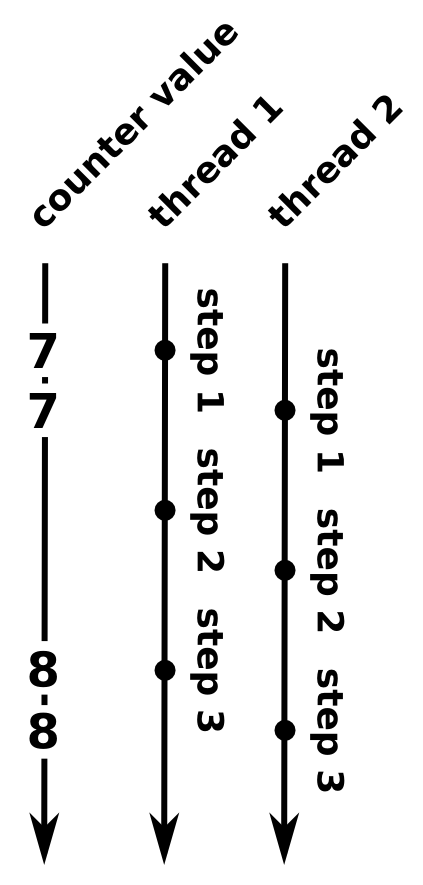
\includegraphics[width=0.23\linewidth]{time_mutable.png}
%% \end{frame}

%% \begin{frame}[fragile]
%% \frametitle{Monoids for combining results}

%% A monoid is a group without inverses:
%% \begin{itemize}
%% \item an identity: $0$ for which $a + 0 = a$
%% \item an associative operator: $a + (b + c) = (a + b) + c$
%% \end{itemize}

%% \vspace{0.2 cm}
%% \mbox{ } \hfill 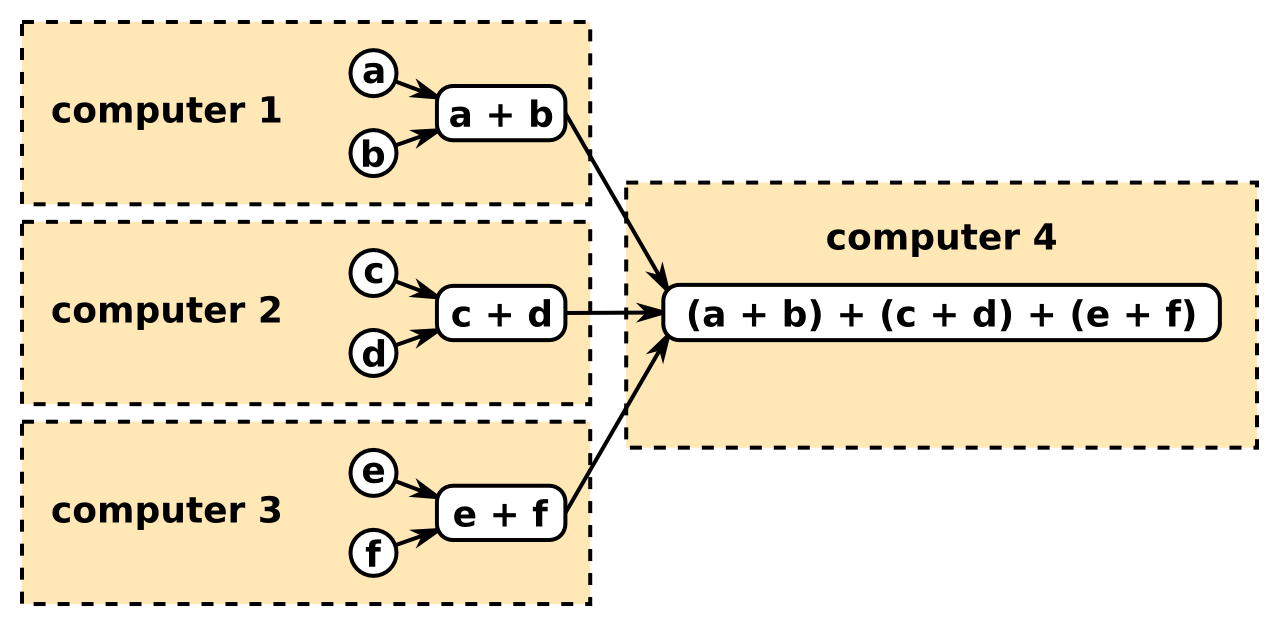
\includegraphics[width=0.7\linewidth]{monoids.png} \hfill \mbox{ }

%% \vspace{0.2 cm}
%% \begin{lstlisting}
%% @case class Ratio(numer, denom):
%%     def add(self, other):
%%         return >Ratio>(self.numer + other.numer,
%%                      self.denom + other.denom)
%%     def value(self):
%%         return self.numer / self.denom
%% \end{lstlisting}
%% \end{frame}

%% \begin{frame}{Language choices for projects I was involved in}
%% \begin{itemize}
%% \item Credit card company: SAS and Python ({\it pure} Python, not even Numpy).

%% \item Web advertising start-up: Python.

%% \item NASA (open source Project Matsu): Java simply because it was a new project using Hadoop and HBase. I think they ordinarily use C++ for image processing.

%% \item Monitoring auto traffic: real-time analysis in Storm (which is in Clojure, a JVM language, but I wrote my code in Scala).

%% \item Auto insurance: SQL over Hadoop, using Hive and Pig. User-defined functions were in Java because Hive and Pig (and Hadoop) are Java.

%% \item Military project: extremely Java-centric.

%% \item Data science start-up: most data analyses in R, a little in Python, but the production data pipeline was strictly Java.
%% \end{itemize}
%% \end{frame}

%% \begin{frame}{Language choice}
%% Based on Google searches for language + ``tutorial'' (log scale).

%% 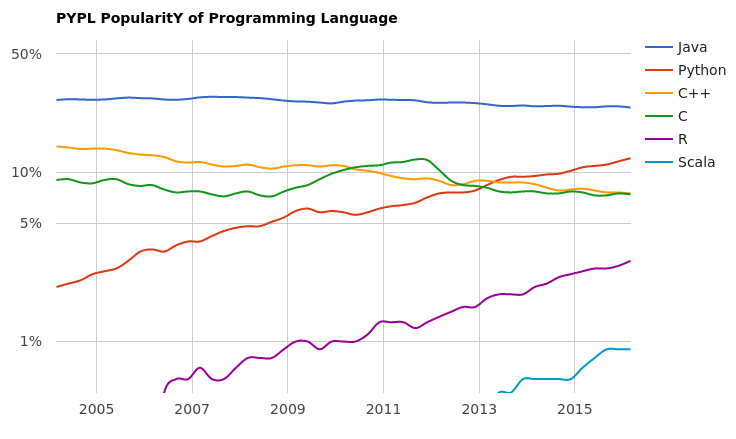
\includegraphics[width=\linewidth]{language_trends.png}
%% \end{frame}

%% \begin{frame}{Major frameworks}
%% \begin{block}{Apache Hadoop}
%% Performs map-reduce calculations. Used as a foundation for other big data frameworks because of\ldots
%% \begin{itemize}
%% \item the HDFS distributed filesystem (even variants like MapR, which don't use HDFS, provide an HDFS API),
%% \item suite of InputFormats that split files by logical records,
%% \item ZooKeeper, which coordinates job configuration and synchronization for any service across a cluster.
%% \end{itemize}
%% \end{block}

%% \begin{block}{Apache Spark}
%% Generalizes from map-reduce to arbitrary pipelines, optimized for iterative procedures, with an interactive prompt. May be used on any cluster manager, but usually Hadoop.
%% \begin{itemize}
%% \item User interfaces: native Scala, Java, Python (through sockets), and R (through pipes).
%% \end{itemize}
%% \end{block}
%% \end{frame}

%% \begin{frame}{Major frameworks}
%% \textcolor{darkblue}{Google Trends result}

%% (frequency of use as a search term, in ``software'' context)

%% 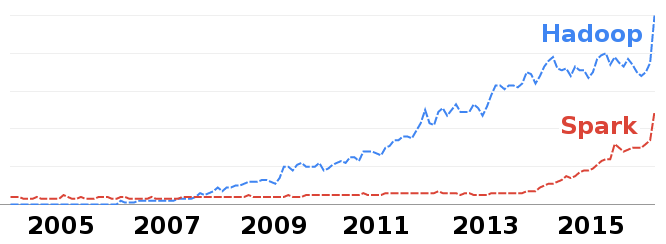
\includegraphics[width=\linewidth]{trends.png}
%% \end{frame}

%% \begin{frame}{Generic data formats}

%% It's also not uncommon to mix file formats and use a lot of text-based formats. Perhaps 70\% of what I saw was JSON.

%% \begin{description}
%% \item[CSV] table of primitives: numbers, booleans, strings (text).
%% \item[JSON] arrays and maps of primitives (text).
%% \item[XML] structures with an optional schema (text).
%% \item[Apache Avro] JSON-like binary format with algebraic data types (arrays, maps, records, and unions of primitives). Similar to \textcolor{darkblue}{Thrift} and \textcolor{darkblue}{Protocol buffers}.
%% \item[Parquet] similar to Avro, but stored column-wise for speed. Similar to \textcolor{darkblue}{ORC}, Hive's format for SQL tables.
%% \item[Sequence files] structured container of arbitrary binary blobs intended as splitting hints for Hadoop.
%% \item[Intermediate serialization in Hadoop and Spark] using native Java serialization, Kryo, and Hadoop Writables.
%% \item[Python pickle files] for persisting Python objects.
%% \end{description}

%% \ldots and many application-specific formats.
%% \end{frame}

%% \begin{frame}[fragile]{Spark's functional primitives in \only<1>{C++}\only<2>{Scala} type syntax}
%% \small
%% \begin{onlyenv}<1>
%% \begin{verbatim}
%% iterator<X> filter(iterator<X>, function<bool(X)>);
%% iterator<Y> map(iterator<X>, function<Y(X)>);
%% iterator<Y> flatten(iterator<iterator<Y>>);
%% iterator<Y> flatMap(iterator<X>, function<iterator<Y>(X)>);

%% Y reduce(iterator<Y>, function<Y(Y,Y)>);      // sum, max, etc.
%% Z aggregate(iterator<Y>, Z, function<Z(Y,Z)>);   // more general

%% map<K,array<V>> groupByKey(iterator<pair<K,V>>); // like SQL's

%% map<K,V> reduceByKey(iterator<pair<K,V>>,     // input data
%%                      function<V(V,V)>);       // merge

%% map<K,Z> aggregateByKey(iterator<pair<K,V>>,  // input data
%%                         Z,                    // starting value
%%                         function<Z(V,Z)>,     // increment
%%                         function<Z(Z,Z)>);    // combine
%% \end{verbatim}
%% \end{onlyenv}
%% \begin{onlyenv}<2>
%% \begin{verbatim}
%% def filter(in: Iterator[X], f: X => Boolean): Iterator[X]
%% def map(in: Iterator[X], f: X => Y): Iterator[Y]
%% def flatten(in: Iterator[Iterator[Y]]): Iterator[Y]
%% def flatMap(in: Iterator[X], f: X => Iterator[Y]): Iterator[Y]

%% def reduce(in: Iterator[Y], f: (Y,Y) => Y): Y
%% def aggregate(in: Iterator[Y], zero: Z, f: (Y,Z) => Z): Z

%% def groupByKey(in: Iterator[(K,V)]): Map[K,Seq[V]]

%% def reduceByKey(in: Iterator[(K,V)],
%%                 merge: (V,V) => V): Map[K,V]

%% def aggregateByKey(in: Iterator[(K,V)],
%%                    zero: Z,
%%                    incr: (V,Z) => Z,
%%                    comb: (Z,Z) => Z): Map[K,Z]
%% \end{verbatim}
%% \end{onlyenv}

%% \normalsize
%% Hadoop's ``mappers'' are actually {\tt flatMap} (which includes the possibility of filtering) and its ``reducers'' are {\tt aggregateByKey}.
%% \end{frame}

%% \begin{frame}[fragile]{Example of using primitives}
%% Suppose we want to fill histograms of $p_T$ for tracks with {\tt fValid} from events with {\tt fTemperature > 20}, with one histogram for each distinct combination of {\tt fTriggerBits}.

%% \begin{onlyenv}<1>
%% \vspace{0.2 cm}
%% On the Spark prompt (Scala syntax):
%% \begin{verbatim}
%% val dataset = sc.rootRDD[Event]("root://fnal.gov/*.root")
%% val histograms =
%%   dataset.filter(event => event.fTemperature > 20)
%%          .flatMap(event => event.fTracks)
%%          .filter(track => track.fValid)
%%          .map(t => (t.fTriggerBits,
%%                     Math.sqrt(t.fPx*t.fPx + t.fPy*t.fPy)))
%%          .aggregateByKey(new TH1F(100, 0, 30))(
%%                          (pt, hist) => hist.Fill(pt),
%%                          (h1, h2) => h1.Add(h2))
%% \end{verbatim}
%% \end{onlyenv}
%% \begin{onlyenv}<2>
%% \vspace{0.2 cm}
%% On the PySpark prompt (Python syntax):
%% \begin{verbatim}
%% dataset = sc.rootRDD("root://fnal.gov/*.root")
%% histograms =
%%   dataset.filter(lambda event: event.fTemperature > 20)
%%          .flatMap(lambda event: event.fTracks)
%%          .filter(lambda track: track.fValid)
%%          .map(lambda t: (t.fTriggerBits,
%%                          math.sqrt(t.fPx**2 + t.fPy**2)))
%%          .aggregateByKey(TH1F(100, 0, 30),
%%                          lambda pt, hist: hist.Fill(pt),
%%                          lambda h1, h2: h1.Add(h2))
%% \end{verbatim}
%% \end{onlyenv}

%% This process gets distributed over the cluster and returns its result to the user's \only<1>{Spark}\only<2>{PySpark} interactive session.
%% \end{frame}

%% KDNuggets
%% Hadoop/Big Data Tools

%% Hadoop/Big Data tool usage jumped to 29% among voters, up from 17% in 2014, and 14% in 2013.
%% This is probably due to availability and low-cost of many cloud-based Big Data tools. Very notable is the jump in Spark share to 11.3%.

%% However, most data analysis is still done on "medium" and small data.

%% Top Hadoop/Big Data tools were

%% Hadoop, 18.4% share (507 votes)
%% Spark, 11.3% (311)
%% Hive, 10.2% (282)
%% SQL on Hadoop tools, 7.2% (198)
%% Pig, 5.4% (150)
%% HBase, 4.6% (127)
%% Other Hadoop/HDFS-based tools, 4.5% (125)
%% MLlib, 3.3% (91)
%% Mahout, 2.8% (76)
%% Datameer, 0.8% (23)

\end{document}
